\section{模拟原理简介和国内外研究现状}
\par{本章主要介绍了吸附扩散理论和计算机分子模拟中常见的模拟方法及其原理,结合国内外学者对于有机分子在H-ZSM-5分子筛上的吸附及扩散的研究结果,对脂肪酸甲酯在H-ZSM-5分子筛上吸附与扩散的科研前景进行展望。}
\subsection{H-ZSM-5分子筛简介}
\par{分子筛是一种含有特殊孔道结构的硅铝酸盐晶体材料,孔径相当于分子尺度大小\cite{1991Zeolite}。它耐高温,吸附能力和择形性强,并被广泛应用于有机化工和石油化工\cite{1999中国土木建筑百科辞典}。分子筛以其孔道直径分类,可分为小孔、中孔和大孔\cite{黄孟凯2013稠环芳烃在},具体差异见\reftab{fenzishai}。}
\begin{table}[htbp]
	\small
	\centering
	\caption{分子筛种类表}
	\begin{tabular}{p{3cm}<{\centering}p{5cm}<{\centering}p{3cm}<{\centering}}
        \toprule
        分子筛种类&\makecell{\ch{TO_4}个数\\(T代表Si或者Al)}&孔径(nm)\\
        \midrule
        小孔&8&<2\\
        中孔&10&2$\sim$50\\
        大孔&12&>50\\
		\bottomrule
	\end{tabular}
	\label{fenzishai}
\end{table}
\par{本文模拟中使用的分子筛为 H-ZSM-5 分子筛。ZSM-5分子筛是一种微孔分子筛,它由正弦孔道和直孔道相互交叉构成,正弦孔道孔径为0.55nm×0.51nm,直孔道孔径为0.53nm×0.56nm\cite{baerlocher2007atlas}。\reffig{fig:H-ZSM-5}展示了H-ZSM-5分子筛的直孔道和正弦孔道结构,其中黄色原子代表Si,红色原子代表O,紫色原子代表Al,白色原子代表H。}
\begin{figure}[H]
    \centering

    \subfigure[正弦孔道]{
    \begin{minipage}[t]{0.5\linewidth}
    \centering
    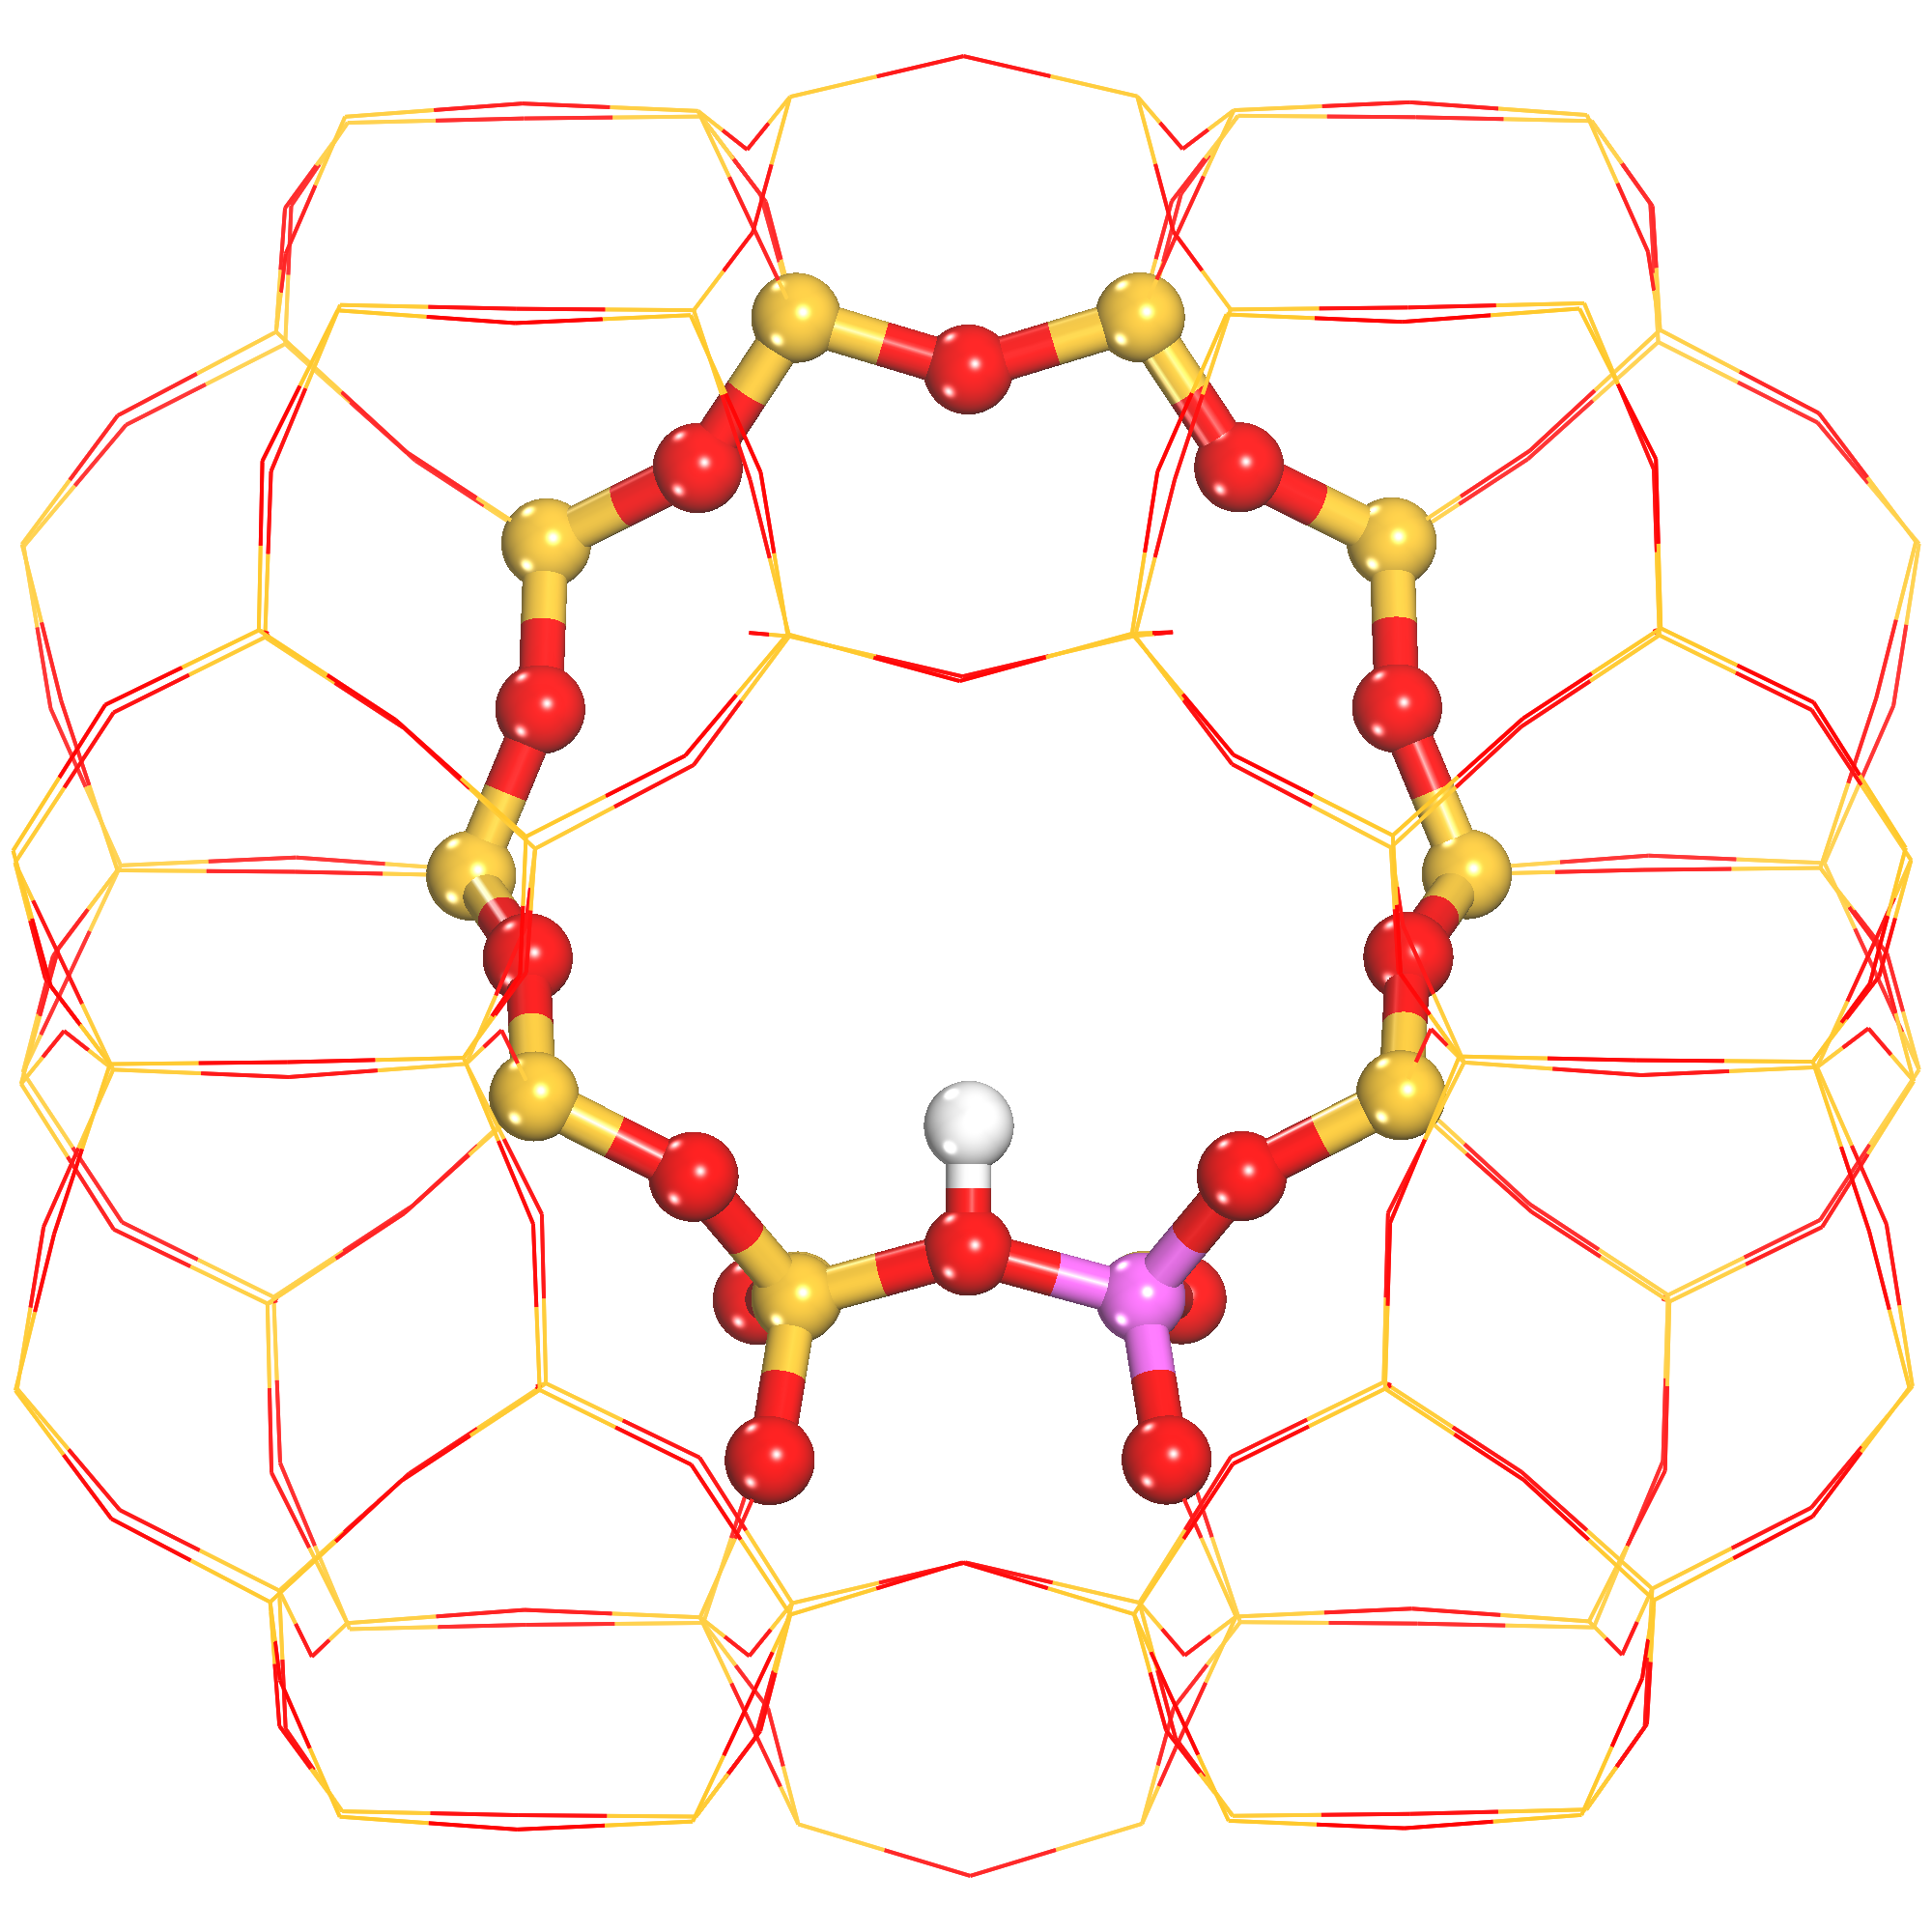
\includegraphics[width=2in]{figure/zigzag.png}
    \end{minipage}%
    }%
    \subfigure[直孔道]{
    \begin{minipage}[t]{0.5\linewidth}
    \centering
    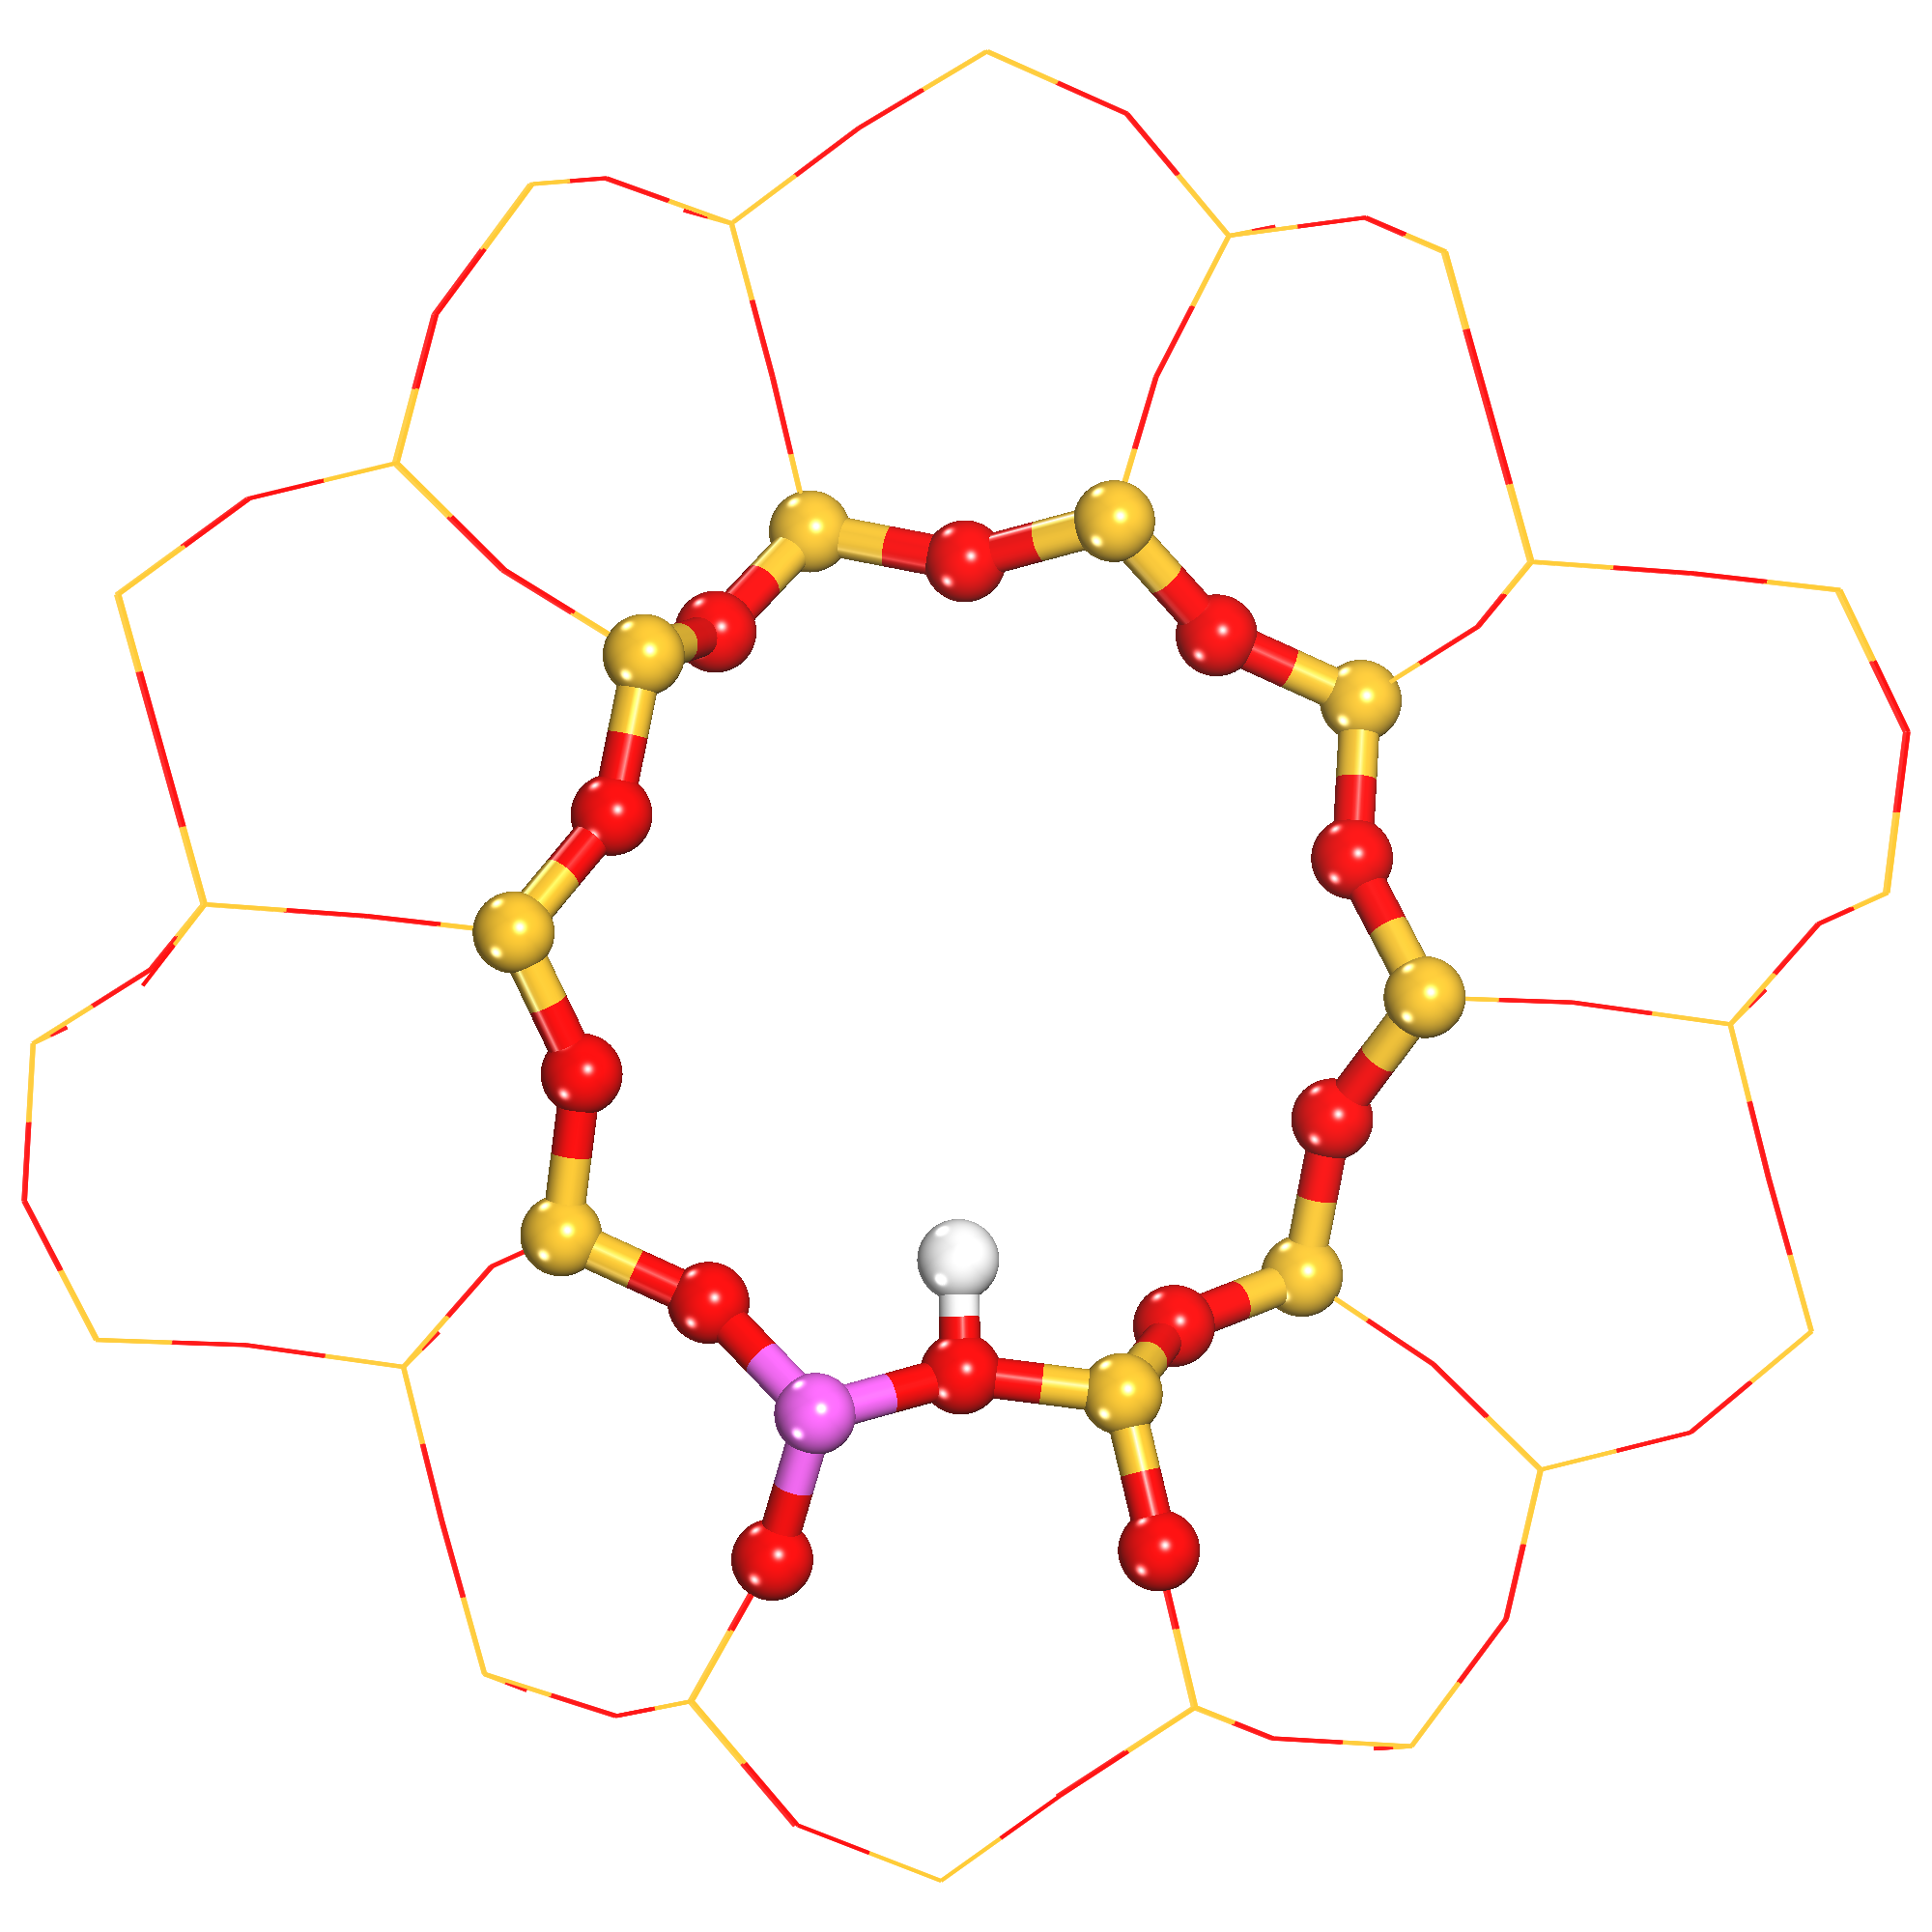
\includegraphics[width=2in]{figure/straight.png}
    %\caption{fig2}
    \end{minipage}%
    }%
    \caption{H-ZSM-5分子筛孔道结构图}
    \label{fig:H-ZSM-5}
\end{figure}
\par{铝原子常被用来取代分子筛骨架上的硅原子,从而形成具有催化活性的质子型或金属离子型分子筛\cite{2013H}。H-ZSM-5分子筛是 ZSM-5 分子筛经过多次铵离子交换处理后,经烘干焙烧得到的 H 型分子筛。H-ZSM-5分子筛的催化活性主要来自Si、Al桥位氧原子质子化所形成的B酸。氢原子除了是反应的活性中心外,也有平衡分子筛电荷的作用。因为H-ZSM-5分子筛在晶体结构、化学组成及物化性质方面具有许多独特性,因此在许多有机催化反应中展现出了优异的催化效果,在工业上得到了越来越广泛地应用\cite{赵振华1985石油化工的新型催化剂——}。}

\subsection{吸附理论}
\subsubsection{吸附简介}
\par{吸附是一种质量传递过程,物体中所有的分子之间都存在互相吸引的力,但在物体表面,内部的分子浓度远大于外部的,表面的分子对物体外部的分子的吸引力没有完全发挥,所以固体的表面可以吸附其他分子。其中吸附剂是具有吸附能力的物质,吸附质是被吸附剂吸附的物质。}
\subsubsection{吸附分类}
\par{吸附按照吸附质与吸附剂间相互作用力性质的差别可以分为化学吸附和物理吸附两大类,具体差异见\reftab{xifu}。}
\begin{table}[htbp]
	\small
	\centering
	\caption{物理吸附和化学吸附对比表}
    \begin{tabular}{p{3cm}<{\centering}p{4cm}<{\centering}p{4cm}<{\centering}}
        \toprule
        吸附类型&物理吸附&化学吸附\\
        \midrule
        作用力&	范德华力	&化学键,电子得失\\
热效应	&近似于凝缩热加润湿热	&近似于化学反应热\\
吸附方式	&单分子层或多分子层	&一般为单分子层\\
解吸结果	&吸附质能还原	&吸附质不能还原\\
吸附过程	&可逆&	不可逆\\
		\bottomrule
	\end{tabular}
	\label{xifu}
\end{table}
\par{本文中的脂肪酸甲酯在 H-ZSM-5 分子筛的吸附属于物理吸附。物理吸附也被称为范德华吸附,它是由吸附剂和吸附质之间的范德华力所引起的。因为任何两个分子间都存在范德华力,所以任何固体表面上都可以发生物理吸附。由于物理吸附是分子间的引力所引起的吸附,所以吸附质与吸附剂之间的作用较弱,于是吸附热较小,吸附和解吸速度也都较快,吸附质容易解吸出来,在一定程度上是可逆的。}
\subsubsection{吸附等温线}
\par{吸附现象的特性包括吸附强度、吸附量、吸附状态等, 而吸附等温线则是宏观地总括这些特性的物理量。吸附等温线是指在一定温度下吸附剂分子在两相的界面上吸附解吸过程达到动态平衡时压力和吸附量之间的关系曲线。}
\par{国际应用化学联合会(IUPAC)根据吸附量随压力的变化将吸附曲线分为以下五种类型:}
\begin{figure}[H]
    \centering

    \subfigure[\uppercase\expandafter{\romannumeral1}型]{
    \begin{minipage}[t]{0.3333\linewidth}
    \centering
    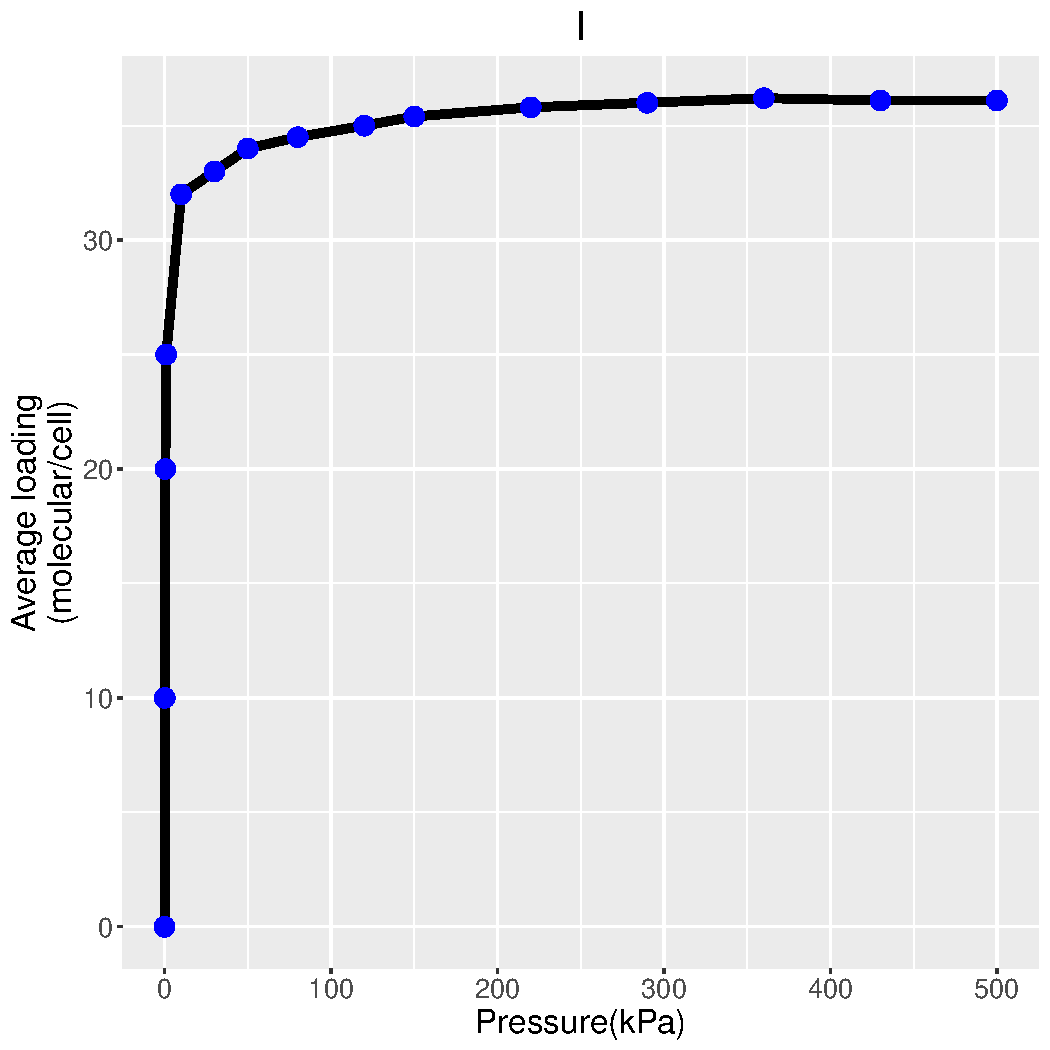
\includegraphics[width=1.8in]{figure/1.pdf}
    %\caption{fig1}
    \end{minipage}%
    }%
    \subfigure[\uppercase\expandafter{\romannumeral2}型]{
    \begin{minipage}[t]{0.3333\linewidth}
    \centering
    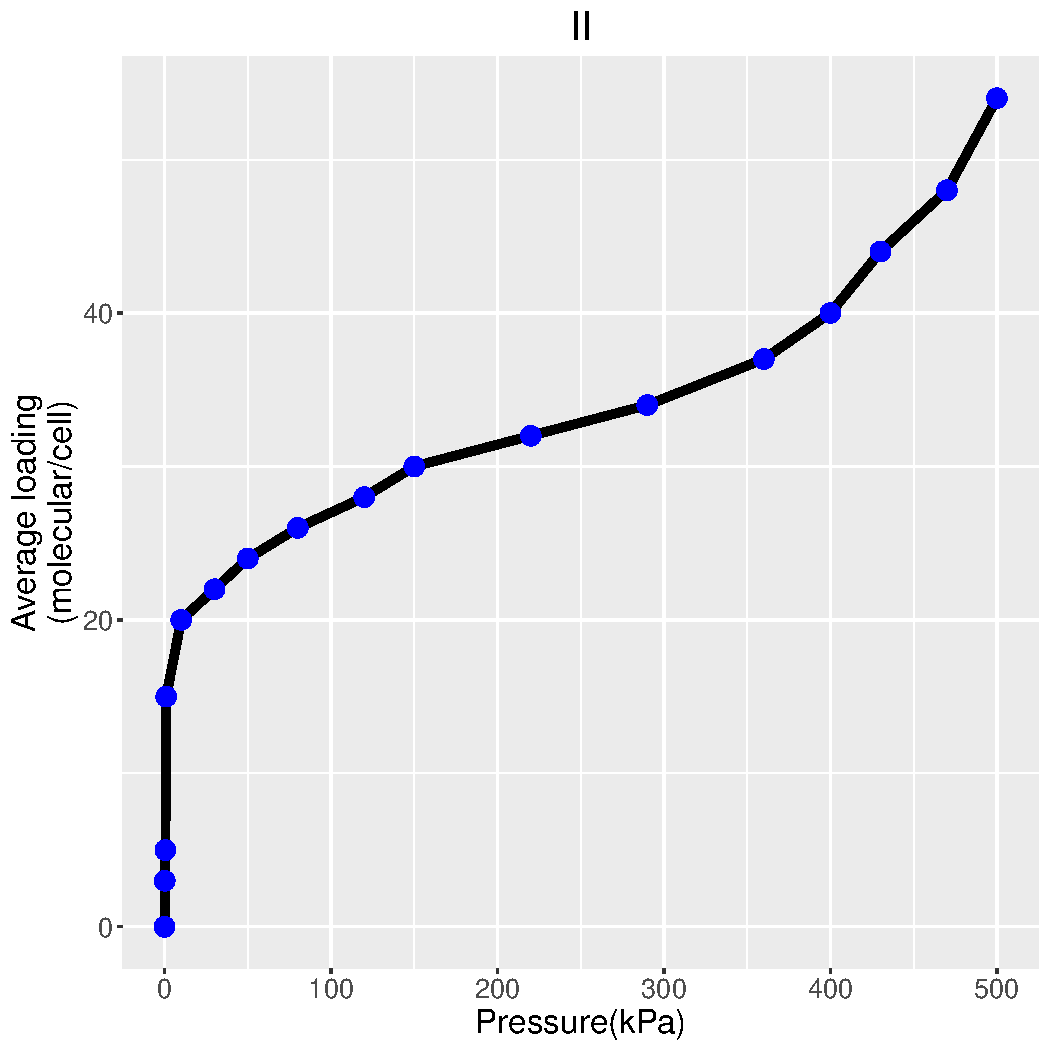
\includegraphics[width=1.8in]{figure/2.pdf}
    %\caption{fig2}
    \end{minipage}%
    }%
    \subfigure[\uppercase\expandafter{\romannumeral3}型]{
    \begin{minipage}[t]{0.3333\linewidth}
    \centering
    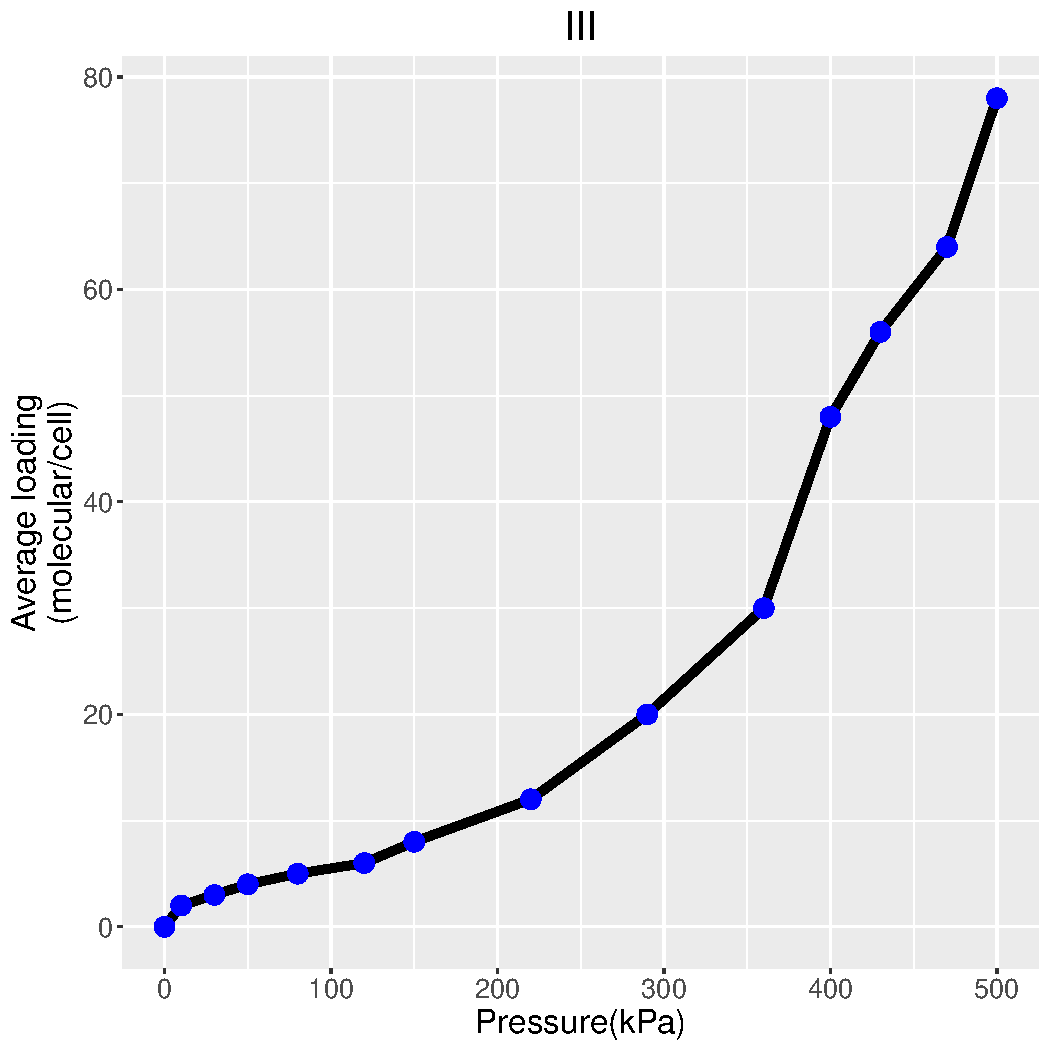
\includegraphics[width=1.8in]{figure/3.pdf}
    %\caption{fig2}
    \end{minipage}%
    }%

    \subfigure[\uppercase\expandafter{\romannumeral4}型]{
    \begin{minipage}[t]{0.3333\linewidth}
    \centering
    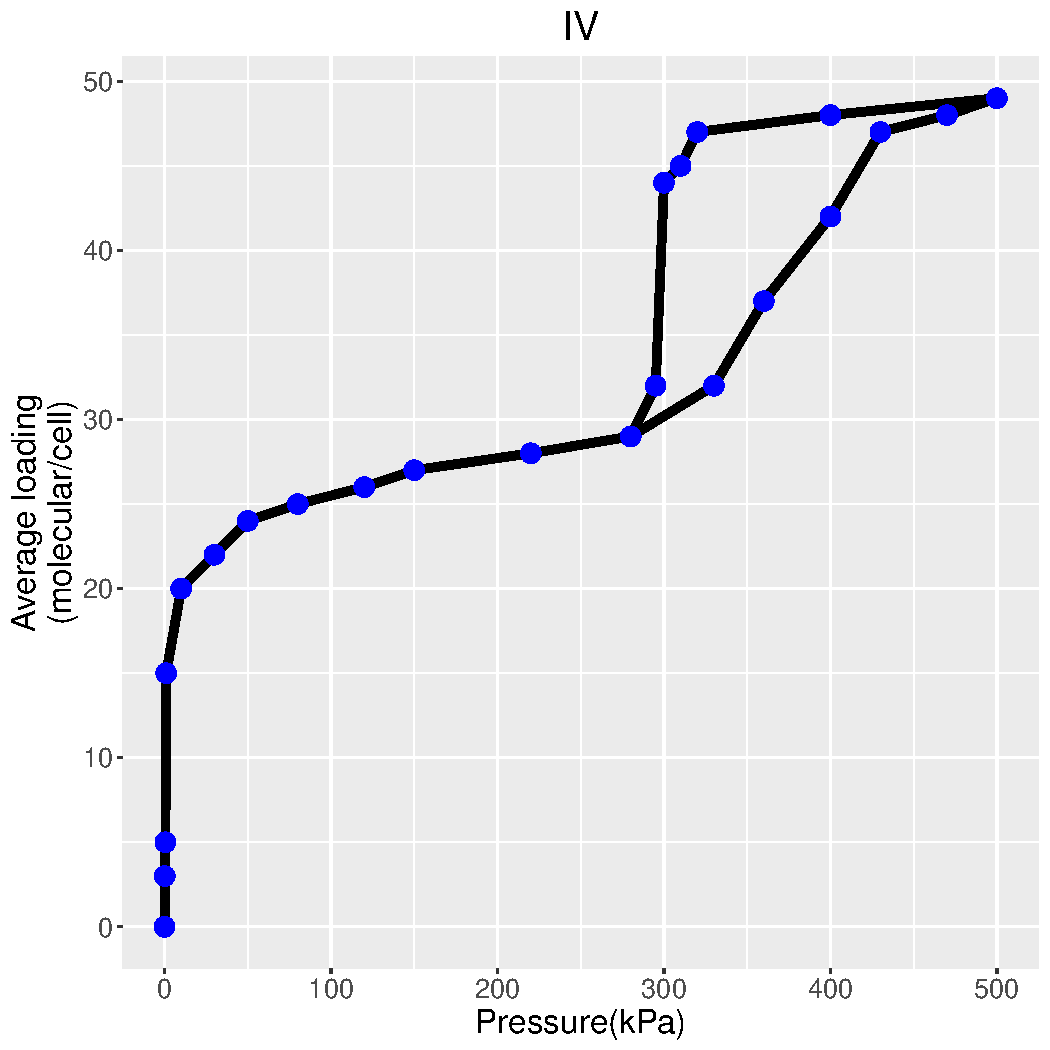
\includegraphics[width=1.8in]{figure/4.pdf}
    %\caption{fig2}
    \end{minipage}%
    }%
    \subfigure[\uppercase\expandafter{\romannumeral5}型]{
    \begin{minipage}[t]{0.3333\linewidth}
    \centering
    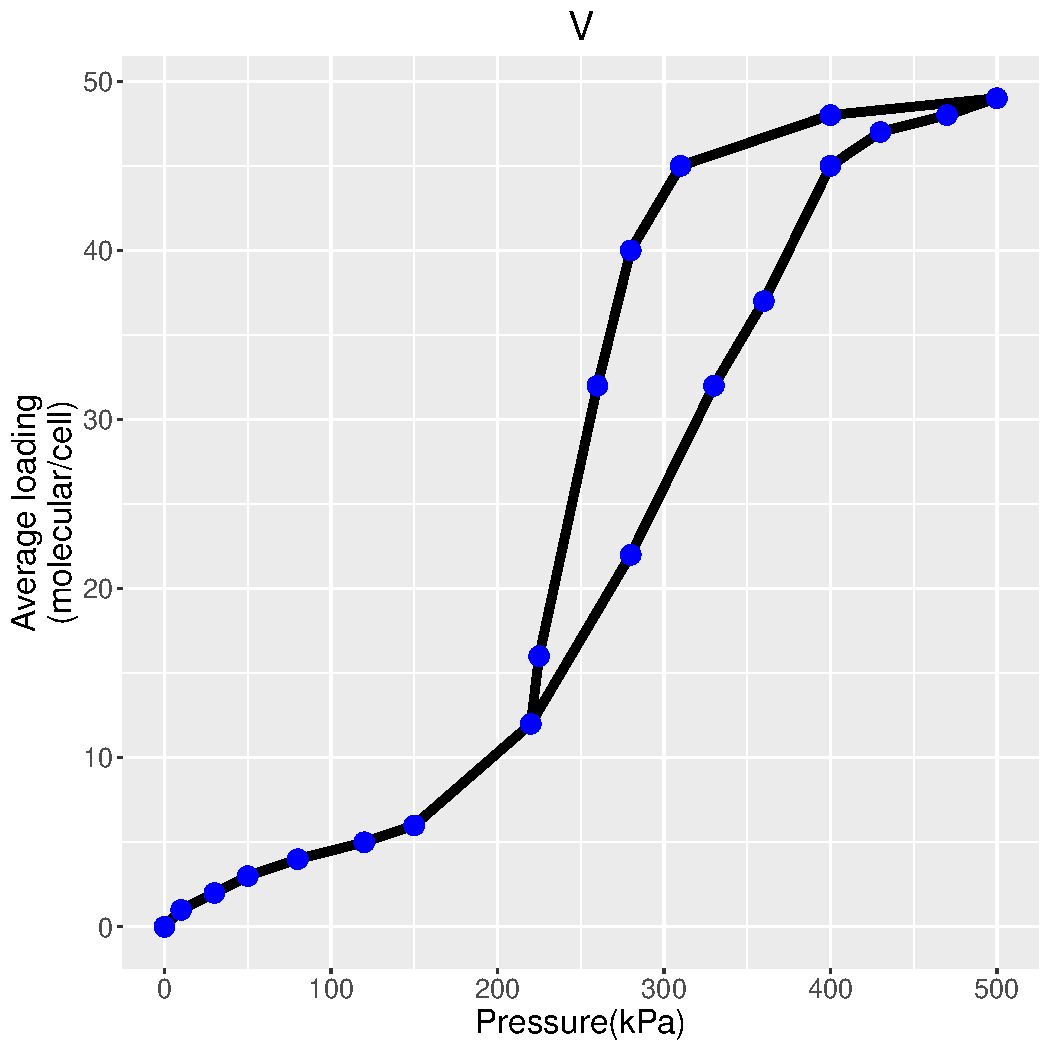
\includegraphics[width=1.8in]{figure/5.pdf}
    %\caption{fig2}
    \end{minipage}%
    }%
    \caption{不同类型的吸附等温线图}
    \label{fig:xifu}
\end{figure}
\subparagraph{Ⅰ型:}
\par{一般反映单分子层可逆吸附,又被称为郎格缪尔等温吸附线。在微孔吸附剂上的吸附等温线一般是这种类型。}
\subparagraph{Ⅱ型:}
\par{一般反映多分子层强吸附。吸附质与吸附剂之间的作用力较大,在较低的压力下吸附量快速增加。拐点处表示单分子层达到吸附饱和,多层吸附随压力的增加逐渐形成,在达到饱和蒸汽压时可近似认为有无限多吸附层。}
\subparagraph{Ⅲ型:}
\par{一般反映多分子层弱吸附。因为吸附质的冷凝热比吸附热还大,所以在高压下吸附速度大于低压下的吸附速度。}
\subparagraph{Ⅳ型和Ⅴ型:}
\par{通常认为是发生了毛细管冷凝后的Ⅱ型和Ⅲ型吸附的变形。}
\subsubsection{郎格缪尔方程}\label{郎格缪尔吸附}
\par{在一定温度下, 吸附质在两相中的浓度关系可用吸附方程式来表示\cite{吴焕领2006吸附等温线的介绍及应用}。朗格缪尔方程是最常用的吸附等温线方程之一,是由物理化学家朗格缪尔 (Langmuir Itying) 根据分子运动理论和一些假定推导出来的,现在被广泛应用于吸附学领域。朗格缪尔认为吸附剂表面的粒子存在向外的剩余价力,它可以吸附气体分子,而这种剩余价力的作用范围与分子直径相当,所以吸附剂表面只能发生单分子层吸附。}
\par{郎格缪尔吸附存在四个假设:}
\begin{enumerate}
    \item 吸附剂的吸附位点只存在于表面,且每个吸附位点只能吸附单个分子;
    \item 吸附剂表面是均匀的,表面上各位点发生吸附的吸附热相同;
    \item 吸附质分子之间的作用力远小于吸附质与吸附剂间的作用力,可以忽略;
    \item 吸附的同时也存在脱附,吸附平衡是动态平衡。
\end{enumerate}
\par{根据上面的假设,可以推导出朗格缪尔吸附方程:}
\par{对于任意吸附过程,均存在如下平衡:}
\begin{equation}
    X(g)+Y(s) \xleftrightarrow[k_{-1}]{k_1} X Y
\end{equation}
\par{式中:$X(g)$ 表示吸附质;$Y(s)$ 表示吸附剂; $k_1$为吸附速率常数;$k_{-1}$ 为解吸速率常数。}
\par{吸附速率表示为:}
\begin{equation}
    V_{1}=k_{1} P(1-\theta) N
\end{equation}
\par{式中:$V_{1}$表示吸附速率;$P$ 为压力; $\theta$为覆盖率; $N$为吸附数。}
\par{解吸速率表示为:}
\begin{equation}
    V_{-1}=k_{-1} \theta N
\end{equation}
\par{式中:$V_{-1}$ 为解吸速率。}
\par{当达到饱和吸附量时,吸附和解吸达到动态平衡,即$V_{1}=V_{-1}$,所以:}
\begin{equation}
    \theta=\frac{b P}{1+b p}
\end{equation}
\par{式中:}
\begin{equation}
    b=\frac{k_{1}}{k_{-1}}
\end{equation}
\par{因为假设吸附为单分子层吸附,而$\theta$为覆盖率,故设:}
\begin{equation}
    \theta=\frac{V_{\mathrm{m}}}{V_{\mathrm{m}^{a}}}
\end{equation}
\par{式中:$V_{\mathrm{m}}$为平衡吸附量;$V_{\mathrm{m}^{a}}$ 为饱和吸附量。}
\par{故:}
\begin{equation}
    V_{\mathrm{m}}=V_{\mathrm{m}^{\mathrm{a}}} \frac{b P}{1+b P}
\end{equation}
\subsection{扩散理论}
\subsubsection{扩散简介}
\par{物质分子从浓度高的地方向浓度低的地方进行转移,直到体系浓度均匀分布的现象叫扩散\cite{2014半无限大体广义电磁热弹扩散问题的动态响应}。扩散由不同区域之间的温度差或者浓度差引起,可以发生在一种或几种物质在同一相态或不同相态之间,直到同一相态内各区域各种物质的浓度均匀或者两相间各种物质的浓度平衡为止。}

\subsubsection{菲克定律}
\par{菲克定律描述的是化工“三传一反”中的质量传递现象。菲克定律是指在不依靠宏观的混合作用发生的传质现象时,描述分子扩散过程中质量通量与浓度梯度之间关系的定律。它包括两个内容:}
\subparagraph{菲克第一定律:}
\par{在单位时间内通过垂直于扩散方向的单位截面积的扩散流量与该截面处的浓度梯度成正比。公式表达为:}
\begin{equation}
    J=-D \dfrac{\partial C}{\partial X}
    \end{equation}
\par{式中:$J$为扩散通量;$D$为扩散系数;$C$为扩散物质的体积浓度;$\dfrac{\partial C}{\partial X} $为浓度梯度;负号表示扩散方向与浓度梯度的方向相反。}
\subparagraph{菲克第二定律:}
\par{在非稳态扩散过程中,$X$ 处的浓度随时间的变化率$\dfrac{\partial C}{\partial t}$ 等于该处的扩散通量随距离变化率的相反数。公式表达为:}
\begin{equation}
    \frac{\partial C}{\partial t}=\frac{\partial \frac{\partial C}{\partial X}}{\partial X}\xrightarrow{\mbox{D不随X变化}}D \frac{\partial^{2} C}{\partial X^{2}}
\end{equation}
\subsubsection{扩散系数}
\par{扩散系数(菲克定律中的$D$)是指在单位时间单位浓度梯度下,沿扩散方向且垂直于单位面积所传递的质量或物质的量。扩散系数主要受扩散物质的物性、压力和温度的影响。}
\par{多年来众多学者都致力于研究扩散物质在分子筛中的扩散机理以及如何测定扩散系数。目前实验测定扩散系数有多种方法:Tezel\cite{tezel1991effect}等人用重量法测定了氮气在分子筛上的扩散动力学;Zhu\cite{zhu2004concentration}等人采用零长度色谱法研究了异丁烷在分子筛上的脱附;卢洪\cite{卢洪2000炭分子筛上氧、氮吸附特性的实验测定}等人用气相色谱法测定了氮气和氧气在分子筛上的扩散系数。而随着计算机技术的发展,分子模拟技术已经被广泛应用在分子筛上的扩散行为的研究\cite{陈玉平2007烷烃在分子筛孔中吸附和扩散的分子模拟,袁帅2011芳烃、环烷烃分子在,杨超2006甲苯歧化反应物与产物在}。}
\subsection{分子模拟理论和方法简介}
\par{分子模拟所依据的理论主要包括经典力学(CM)和量子力学(QM)。常用的经典力学方法主要有:分子力学方法(MM)、蒙特卡罗方法(MC)和分子动力学方法(MD)。常用的量子力学方法有:半经验算法(Semi-empirical Method),从头算方法(Ab initio Method)以及密度泛函理论(Density Functional Theory)\cite{刘丹2004分子模拟在分子筛催化研究中的应用}。}
\par{与实验相比,利用计算机研究化学现象的方法有下列几项优点\cite{分子模拟的理论与实践}:}
\begin{enumerate}
    \item 降低研究成本;
    \item 增加安全性;
    \item 可研究极快速的反应或变化;
    \item 准确度较高;
    \item 增加对问题的了解。
\end{enumerate}
\par{本文采用的方法主要有分子力学、分子动力学、蒙特卡洛法和密度泛函理论。通过密度泛函理论和分子力学可以得到吸附分子和分子筛的几何优化构象;通过蒙特卡洛法可以得到吸附等温线、吸附热、吸附位点以及吸附质在分子筛中的分布情况;通过分子动力学可得到扩散轨迹和扩散系数。}
\par{下面对所采用的方法以及模拟原理进行简单的介绍。}
\subsubsection{分子力学}
\par{分子力学是在原子、分子水平上用力场解决问题的非量子力学方法\cite{王艺峰2003高分子材料模拟中的分子力学法和力场}。根据波恩-奥本海默近似原理,可以将分子中电子运动的能量忽略,所以体系的能量就是原子核位置的函数。分子力学中的力场中的许多参数可以通过量子力学计算或者实验方法得到,从而避开了考虑电子结构和运动的细节,所以利用分子力学可以计算庞大且复杂的分子的稳定构象、热力学特性和振动光谱等性质\cite{分子模拟的理论与实践}。与量子力学相比,分子力学简单并且可以快速得到分子的各种性质。}
\par{在分子模拟中,合适的力场对于模拟结果的准确性起着决定性作用,它是分子力学方法的核心和关键。通过选取合适的力场就可以计算出分子各种构象的势能,而势能最小的构象就是最稳定的构象。求取势能最低点的过程被称为能量最小化,所得到的构象被称为几何优化构象,它是计算分子物性的基础。本文采用了COMPASS\RNum{2}力场进行模拟。COMPASS\RNum{2}力场能够模拟小分子与高分子,一些金属离子、金属氧化物与金属。在计算有机与无机体系时,采用分类别处理的方式,不同的类别采用不同的模型,即使在计算两种类别的混合体系时,仍然能够采用合理的模型描述\cite{梁太宁2001分子力场},所以COMPASS\RNum{2}力场非常适合本文的脂肪酸甲酯与分子筛体系。其中共价键模型的形式如下:}
\begin{align}
    U &=U_{\mbox{\tiny 键合项}}+U_{\mbox{\tiny 非键合项}}\notag\\
      &=U_{\mbox{\tiny 键合项}}+U_{i, j}+U_{elec}
\end{align}
\begin{align}
    U_{\mbox{\tiny 键合项}} &= U_{b}+U_{\theta}+U_{\phi}+U_{\chi}+U_{cross}\notag\\
      &=\sum_{b}\left[k_{2}\left(b-b_{0}\right)^{2}+k_{3}\left(b-b_{0}\right)^{3}+k_{4}\left(b-b_{0}\right)^{4}\right]\notag\\
      &+\sum_{\theta}\left[k_{2}\left(\theta-\theta_{0}\right)^{2}+k_{3}\left(\theta-\theta_{0}\right)^{3}+k_{4}\left(\theta-\theta_{0}\right)^{4}\right]\notag\\
      &+\sum_{\phi}\left[k_{1}(1-\cos \phi)+k_{2}(1-\cos 2\phi)+k_{3}(1-\cos 3\phi)\right]\notag\\
      &+\sum_{\chi} k_{2} \chi^{2}+\sum_{b, b^{\prime}} k\left(b-b_{0}\right)\left(b-b_{0}^{\prime}\right)+\sum_{b, \theta} k\left(b-b_{0}\right)\left(\theta-\theta_{0}\right)\notag\\
      &+\sum_{b, \phi} \left(b-b_{0}\right)\left[k_{1} \cos \phi+k_{2} \cos 2 \phi+k_{3} \cos 3 \phi\right]\notag\\
      &+\sum_{b^{\prime}, \phi} \left(b^{\prime}-b_{0}^{\prime}\right)\left[k_{1} \cos \phi+k_{2} \cos 2 \phi+k_{3} \cos 3 \phi\right]\notag\\
      &+\sum_{\theta, \phi} \left(\theta+\theta_{0}\right)\left[k \cos \phi+k \cos 2 \phi+k \cos 3 \phi\right]\notag\\
      &+\sum_{\theta^{\prime}, \theta} k\left(\theta^{\prime}-\theta_{0}^{\prime}\right)\left(\theta-\theta_{0}\right)+\sum_{\theta^{\prime}, \theta, \phi} k\left(\theta^{\prime}-\theta_{0}^{\prime}\right)\left(\theta-\theta_{0}\right)\cos \phi
\end{align}
\begin{equation}
    U_{elec}=\sum_{i, j} \frac{q_{i} q_{j}}{r_{i j}}
\end{equation}
\begin{equation}
    U_{i, j}=\sum_{i, j} \varepsilon_{ij}\left[2\left(\frac{r_{i j}^{0}}{r_{i j}}\right)^{9}-3\left(\frac{r_{i j}^{0}}{r_{i j}}\right)^{6}\right]
\end{equation}

\par{式中:$U_{i, j}$是范德华能;$U_{elec}$是库伦能;$U_{b}$是键伸缩能;$U_{\theta}$是键角弯曲能;$U_{\phi}$是键扭转能;$U_{\chi}$是键角面外弯曲能;$U_{cross}$是相互耦合能。}
\par{将分子中各原子核的位置参数带入COMPASS\RNum{2}力场即可得到体系的总能量,再通过最速下降法、共轭梯度法、牛顿拉森法等方法求得该势能函数的最小值和对应的位置参数。通过位置参数,即可得到该分子的几何优化构象。}
\subsubsection{密度泛函理论}
\par{量子力学是以分子中电子的非定域化为基础,认为体系内粒子运动满足薛定谔方程,一切电子的行为以其波函数表示。通过分析分子所表现的性质与其微观结构参数(如电荷密度、轨道、能级等)的关系,而后再根据性质来优化模型结构。理论上讲,量子力学方法几乎可以得到关于分子的一切信息与性质,且结果与实验的结果往往相当吻合。}
\par{密度泛函理论是一种通过研究物质结构统计性的理论,既可以通过量子力学的密度泛函理论研究微观结构,也可以通过统计力学的密度泛函理论研究宏观结构。密度泛函理论都是以密度分布$\rho(r)$作为变量,然后构建密度泛函,它不是某个特定位置的函数,而是函数在整个变量空间中的变化。其中量子力学的密度泛函理论是通过电子的密度分布$\rho(r)$代替波函数$\Psi(\tau)$作为变量,然藏构筑能量的密度泛函,最后应用薛定谔方程求解\cite{密度泛函理论}。薛定谔方程如\refequ{xue1}和\refequ{xue2}所示。}
\begin{equation}\label{xue1}
    -\frac{\hbar^{2}}{2 \mu}\left(\frac{\partial^{2} \Psi}{\partial x^{2}}+\frac{\partial^{2} \Psi}{\partial y^{2}}+\frac{\partial^{2} \Psi}{\partial z^{2}}\right)+U(x, y, z) \Psi=i \hbar \frac{\partial \Psi}{\partial t}
\end{equation}
\begin{equation}\label{xue2}
    -\frac{\hbar^{2}}{2 \mu} \nabla^{2} \Psi+U \Psi=E \Psi
\end{equation}
\par{通过求解薛定谔方程即可求得波函数$\Psi$对应的本征值$E$,即可求得能量。通过比较不同波函数的本征值就可以求得最低能量,而该波函数的坐标参数所对应的结构即是几何优化构象。}
\subsubsection{蒙特卡洛法}
\par{蒙特卡洛方法又被称为随机模拟方法,是一种对构建好的概率模型重复进行大数量的统计模拟,其核心是一种统计方法。在一定系综条件下, 将体系内粒子进行随机的转动、位移或在两相间转移位置,然后运用统计热力学理论进行统计平均,使结果逐渐趋近于平衡时的玻尔兹曼分布,以此获得体系的宏观性质。所以理论上来说,只要有足够多的粒子,就能得到期望的宏观量。该方法最大的优势在于其收敛条件不受问题维数的影响,但由于粒子的位移是计算机随机赋予的,只能在大数量实验结果下反应概率问题,并不能代表粒子的真实运动过程,所以不能用于模拟传递性质\cite{分子模拟技术在石油相关领域的应用}。}
\par{蒙特卡洛方法的模拟过程一般分为如下几步\cite{分子模拟的理论与实践}:}
\begin{enumerate}
    \item 通过随机数发生器生成一个初始的分子构型。
    \item 将这个分子构型中原子的坐标做无规律的改变,生成一个新的分子构型。
    \item 计算出新的分子构型的能量。
    \item 比较原分子构型和新的分子构型的能量大小,判断是否采用新构型。
    \begin{enumerate}[label=(\alph*),leftmargin=2em]
        \item 假如新的分子构型能量小于原分子构型的能量,则接受新的分子构型,并使用这个构型重复再做下一次迭代。
        \item 假如新的分子构型能量大于原分子构型的能量,则计算出玻尔兹曼因子,并生成一个随机数。假如这个随机数大于所计算出的玻尔兹曼因子,则舍弃这个构型,重新计算。若这个随机数小于所计算出的玻尔兹曼因子,则接受这个构型,使用这个构型重复再做下一次迭代。
    \end{enumerate}
    \item 如此进行迭代计算,直至最后得到低于所给能量条件的分子构型为止。
\end{enumerate}
\par{计算吸附性能时采用的是巨正则系综(GCMC),这代表体系的粒子数N不固定,但体系的体积V、化学势μ和温度T不变。利用达到平衡时,吸附剂表面的吸附质的温度和化学势与吸附剂外的相等,从而可以研究在固定温度和压力下吸附质分子在吸附剂内的吸附特性。}
\subsubsection{分子动力学}\label{分子动力学}
\par{分子动力学模拟是一种依靠经典力学来计算经典多体系的平衡过程以及传递性质的模拟方法\cite{分子模拟方法及模拟软件在高分子材料中的应用}。与蒙特卡洛方法相比,分子动力学中的模拟中系统中粒子的运动有正确的物理依据。而且此方法的计算精度性高,可同时获取系统的动态与热力学统计资料。}
\par{分子动力学模拟过程通常遵循以下六个步骤\cite{烷烃分子在MCM-41中吸附和扩散的分子模拟}:}
\begin{enumerate}
    \item 将体系中的粒子看作质点;
    \item 将体系中的所有质点根据玻尔兹曼分布指定初始速度以及初始位置;
    \item 根据所选力场,计算每个质点的势能,确定每个粒子在体系中受到的力;
    \item 根据经典力学,求解运动方程;
    \item 在指定模拟时间内重复步骤(3)和(4);
    \item 将计算结果平均应用到整个体系,确定体系的宏观特性。
\end{enumerate}
\par{通过上面的计算步骤,可以得到体系中所有粒子的扩散轨迹,这些轨迹可以反映出系统中粒子的真实运动状态。以$\vec r_{i}(t)$表示时间$t$时粒子i的位置,粒子位移平方的平均值称为均方位移(MSD),即:}
\begin{equation}
    \mathrm{MSD}=R(t)=\left\langle|\vec{r}(t)-\vec{r}(0)|^{2}\right\rangle
\end{equation}
\par{式中:尖括号表示平均值。}
\par{根据统计的原理,只要有足够多的粒子,足够长的计算时间,系统的任一瞬间都可以当作时间的零点,而所计算的平均值应该相同。假设分子动力学计算共存储了n步轨迹,各步的位置向量分别是$\vec r(1)$、$\vec r(2)$、$\vec r(1)$、……和$\vec r(n)$。在计算均方位移时,每次计算$R(t)$取$n/2$组数据的平均。将轨迹分为:}
$$
\vec{r}(1)\mbox{,}\vec{r}(2)\mbox{,……,}\vec{r}(n / 2)\quad\mbox{及}\quad\vec{r}(n / 2+1)\mbox{,}\vec{r}(n / 2+2)\mbox{,……,}\vec{r}(n)
$$
\par{假设每步的时间间隔为$\delta t$,因为任一瞬间都可以视为零点,所以均方位移为:}
\begin{align}\label{equ:MSD}
    R(\delta t)&=\frac{|\vec{r}(2)-\vec{r}(1)|^{2}+|\vec{r}(3)-\vec{r}(2)|^{2}+\cdots+|\vec{r}(n / 2+1)-\vec{r}(n / 2)|^{2}}{n / 2}\notag\\
    R(2 \delta t)&=\frac{|\vec{r}(3)-\vec{r}(1)|^{2}+|\vec{r}(4)-\vec{r}(2)|^{2}+\cdots+|\vec{r}(n / 2+2)-\vec{r}(n / 2)|^{2}}{n / 2}\notag\\
    &\dots\notag\\
    R(m \delta t)&=\frac{|\vec{r}(m+1)-\vec{r}(1)|^{2}+|\vec{r}(m+2)-\vec{r}(2)|^{2}+\cdots+|\vec{r}(m+n / 2)-\vec{r}(n / 2)|^{2}}{n / 2}\notag\\
    &\dots\notag\\
    R(n \delta t / 2)&=\frac{|\vec{r}(n / 2+1)-\vec{r}(1)|^{2}+|\vec{r}(n / 2+2)-\vec{r}(2)|^{2}+\cdots+|\vec{r}(n)-\vec{r}(n / 2)|^{2}}{n / 2}
\end{align}
\par{\refequ{equ:MSD}是计算一个粒子均方位移的公式,如果要计算系统中所有粒子的均方位移则需要再对粒子数进行平均。\reffig{fig:MSD}展示了LJ势能下的系统的均方位移与时间的曲线。由\reffig{fig:MSD}可知:当时间值很小时,MSD以对数形式增加;当时间值很大时,曲线近似为一条直线。}
\begin{figure}[H]
    \centering
    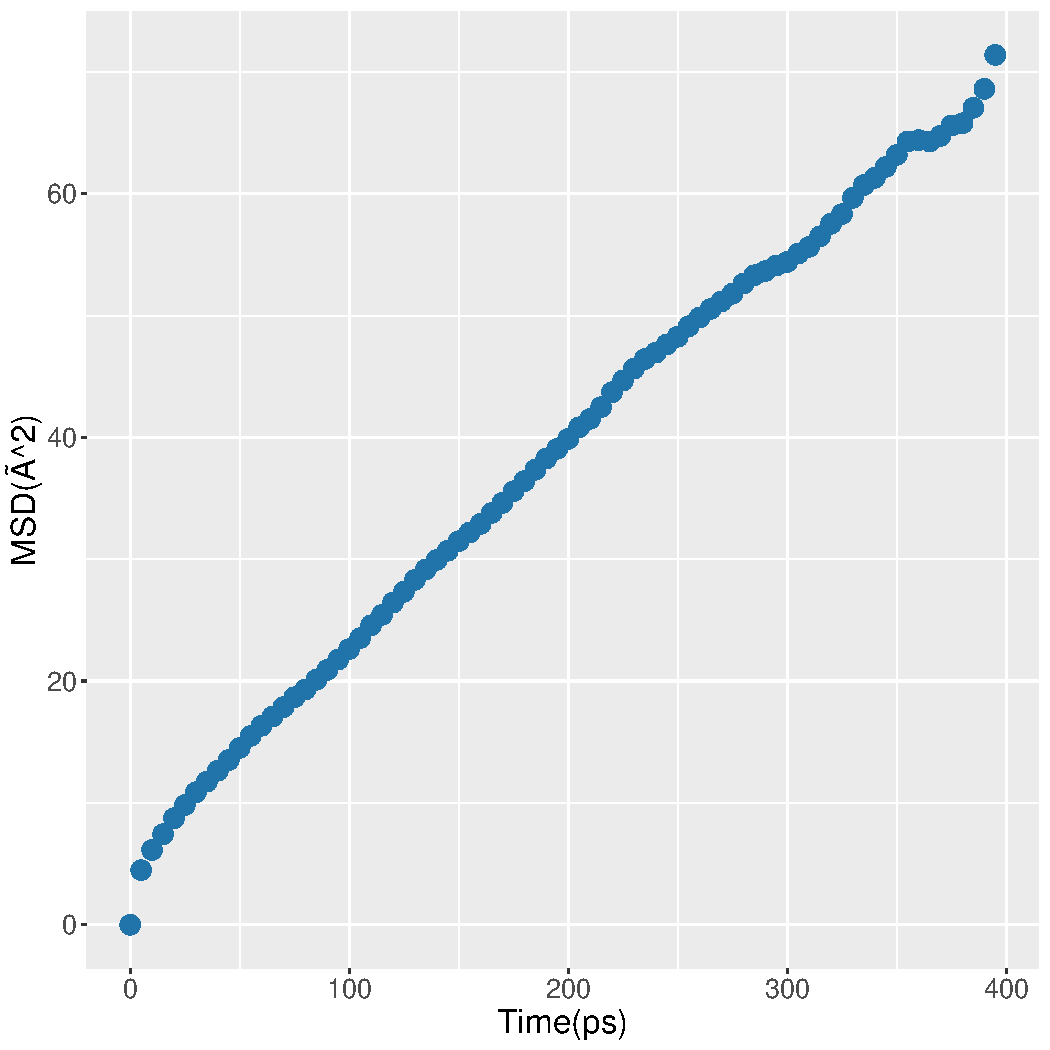
\includegraphics[width=0.5\textwidth]{figure/MSD.pdf}
    \caption{LJ粒子系统的均方位移图}
    \label{fig:MSD}
\end{figure}
\par{根据斯托克斯 - 爱因斯坦方程,有:}
\begin{equation}
    \lim _{t \rightarrow \infty}\left\langle|\vec{r}(t)-\vec{r}(0)|^{2}\right\rangle= 6 D t
\end{equation}
\par{式中:$D$为粒子的扩散系数。}
\par{因此,当计算时间很长时,体系中所有粒子的扩散系数等于均方位移对时间的曲线斜率的六分之一。}
\subsection{国内外研究现状}
\par{本节介绍了目前国内外学者对脂肪酸甲酯在催化裂化和吸附扩散领域的研究成果。讨论在脂肪酸甲酯催化催化裂化工艺中,H-ZSM-5分子筛相较于其他催化剂的优点,确定了催化剂最佳的硅铝比,以及影响吸附扩散性能的因素。}
\subsubsection{脂肪酸甲酯催化裂化工艺研究}
\par{目前许多学者在不同的催化剂上进行了脂肪酸酯的催化裂化反应,所用到的催化剂包括分子筛催化剂和无定型催化剂等。不同的催化剂对脂肪酸酯的催化想产物分布及原料转化率上都有很大的影响。而即使是同一种催化剂,因为催化剂的性质,如孔结构、酸性、择形度,比表面、结晶度等等性质,也都会对反应结果造成很大影响。比如不同的硅铝比会导致催化剂酸性位数量的不同,而催化中间产物会在酸性位上发生二次裂解,从而生成小分子烃类,所以,硅铝比的多少对反应结果的影响尤为重要。本小节主要介绍了催化剂的种类以及硅铝比对脂肪酸甲酯催化裂化的研究。}
\subparagraph{催化剂种类的影响}
\par{Katikaneni\cite{katikaneni_performance_1995}等人研究了在不同温度条件下,不同裂化催化剂上菜籽油的催化转化的产物分布情况。研究结果表明:H-ZSM-5 与其他沸石和非沸石催化剂相比,反应生成的有机液体产品最多,达63 wt\%,而且对芳烃有更高的选择性。Idem\cite{idem_catalytic_1997}等人研究了菜籽油在 H-ZSM-5、硅铝酸盐、二氧化硅、硅氧化铝、γ- 氧化铝、氧化钙和氧化镁催化剂的催化裂化过程。研究结果表明:高择形性的催化剂(如 HZSM-5 和硅铝酸盐催化剂)允许轻微的二次裂化,从而导致低气体产量和高有机液体产品产量。}
\subparagraph{硅铝比的影响}
\par{Dandik\cite{dandik1998catalytic}等人研究了向日葵废油在不同硅铝比的 H-ZSM-5 催化剂上的催化转化。研究结果表明:催化剂中铝的含量越高,反应的转化率越高。Benson\cite{benson2008heterogeneous}等人利用油酸作为不饱和脂肪酸的模型化合物,在H-ZSM-5 催化剂催化下,研究了不饱和脂肪酸催化转化机理。研究结果表明:在高酸性的形状选择催化剂上,可生产多种产品,包括石蜡、烯烃和芳香族化合物。田华\cite{脂肪酸酯的催化裂化研究}在固定床微反应器上进行了脂肪酸酯催化裂化反应的研究。研究结果表明:只要催化剂存在弱酸位,二次裂化反应即可发生;催化剂的酸性越强,二次反应发生的比例越高,生成更多的汽油、液化石油气等小分子;而催化剂上没有酸性位时,二次反应发生较少,液体产物中存在大量的含氧衍生物。Twaiq\cite{twaiq2003liquid}等人研究了棕榈油在以铝硅酸盐介孔材料为催化剂的催化裂化作用。研究结果表明:催化剂活性随铝含量的增加而提高,最终达到最佳水平,而较高的铝含量降低了棕榈油的结晶度,从而降低了棕榈油的催化裂化活性。}
\subparagraph{总结}
\par{ZSM-5 催化剂相比于其他催化剂,因其特有的孔道结构和表面酸性,提高了汽油等产品的收率;H-ZSM-5 催化剂硅铝比越大,酸性越强,二次反应发生的比例越高,就可以生产更多的汽油,减少了含氧衍生物的生成;但铝含量过高,会导致分子筛的热稳定性下降,孔道直径减小;所以适当硅铝比的 H-ZSM-5 分子筛更适合做脂肪酸甲酯催化裂化的催化剂。本文所采用的硅铝比来自Danu\cite{danuthai2009conversion}等人对辛酸甲酯在H-ZSM-5分子筛上的催化裂化实验。}
\subsubsection{脂肪酸甲酯吸附研究}
\par{分子筛的酸性位点不仅是二次催化发生的地方,也是吸附的主要场所之一,而硅铝比的大小会决定分子筛酸性位的数量。如果分子筛孔径过大,虽然吸附分子可以进入分子筛内表面,但这将导致吸附位数量减少,从而影响饱和吸附量,并且孔径大小对吸附能大小也有影响。脂肪酸甲酯催化裂化的原料中既有饱和酯,也有不饱和酯,既有长链,也有短链,所以研究吸附分子的不饱和度和链长因素对吸附的影响对催化剂的设计尤为重要。}
\subparagraph{硅铝比的影响}
\par{洪新\cite{不同硅铝比ZSM-5的合成及其吸附脱除柴油中苯胺和吡啶的性能}等人研究了不同硅铝比的ZSM-5分子筛对柴油中苯胺和吡啶的吸附脱除性能。研究结果表明:硅铝比较小的ZSM-5的吸附脱除苯胺或吡啶的效果明显优于其他样品。}
\subparagraph{孔径大小的影响}
\par{Zhao\cite{zhao2008investigation}等人采用高精度智能重量分析仪,研究了介孔 ZSM-5 结构的扩散和吸附行为。研究结果表明:与在微孔 ZSM-5 相比,引入的介孔降低了4.6倍扩散 - 吸附活化能;因此,尽管在介孔 ZSM-5 催化剂上B酸位降低,但与微孔 ZSM-5 催化剂相比,轻烯烃总收率提高了 2.47 wt\%。Liu\cite{liu2012adsorption}等人采用高精度智能重量分析和零长柱法,研究了在介孔 HZSM-5 分子筛中正辛烷的吸附扩散性能。研究结果表明:与常规 HZSM-5相比,正辛烷在 H-ZSM-5 分子筛中的吸附活化能显著降低;在分子筛中引入介孔为反应物和产物提供了较短的扩散路径和较高的扩散速率,从而提高了燃料油的收率,增强了甲醇与汽油反应中对催化剂失活的抵抗力。}
\subparagraph{不饱和度的影响}
\par{丁雪\cite{Fcc干气在zsm-5分子筛中吸附的分子模拟及热力学分析}等人应用巨正则蒙特卡罗方法(GCMC) 研究了干气中的主要组分在 ZSM-5 分子筛中的吸附行为。研究结果表明:与其它组分相比,乙烯在 ZSM-5 中的吸附量最大。罗演强\cite{生物柴油组分的润滑性能及其在铁表面吸附行为模拟探究}采用 Materials Studio 软件模拟不同酯类在铁表面的吸附行为。研究结果表明:不饱和脂肪酸甲酯具有更强极性的分子的单分子吸附能明显提高。}
\subparagraph{碳链长度的影响}
\par{谭雅文\cite{催化裂化干气组分在ZSM-5中的吸附模拟研究}应用巨正则蒙特卡洛方法(GCMC)进行了干气主要组分在 ZSM-5 中的吸附模拟研究。研究结果表明:C1 $\sim$ C6烷烃的吸附热与氢原子数之间存在线性关系, 并且分子体积越大, 吸附能力越强。Meyer\cite{de2003packing}等人采用间歇吸附技术研究了 C5$\sim$C22 直链烷烃在 ZSM-5 上的液相吸附。研究结果表明:烷烃的饱和容量很大程度上取决于链长。吸附的每单位晶胞 -\ch{C H_x} 基团的数量在 C7 和 C8 之间急剧下降,然后稳定上升,达到 C14$\sim$C22的平稳期。王勇利\cite{C2-6烯烃在h-zsm-5分子筛周期性模型上吸附的理论研究}等人采用密度泛函理论研究了 C2$\sim$C6 直链烯烃在 H-ZSM-5 分子筛上的吸附行为。研究结果表明:对于 C2$\sim$C6 直链烯烃,随着碳数的增加,烯烃的吸附能以 - 12 kJ/mol 的常数线性增大;烯烃在分子筛孔道中吸附时,范德华力起主要作用,碳数增加其影响增大。}
\subparagraph{温度和压力的影响}
\par{李健博\cite{几种气体在ZSM-5分子筛上吸附的模拟与实验研究}分别用实验和模拟的方法,研究了小分子气体在ZSM-5分子筛上的吸附。研究结果表明:四种气体在ZSM-5分子筛上的吸附量随温度的升高而减小,随压力的增大而增加,吸附量随压力的变化规律与实验一致。余英哲\cite{氮气、氩气、氧气在ZSM-5分子筛上吸附的分子模拟研究}等人基于 GCMC 原理,采用分子模拟方法研究了三种小分子气体在 ZSM-5 分子筛上的吸附变化规律。研究结果表明:三种气体的吸附等温线在压力较低的范围,曲线斜率较大,吸附量随压力的增大而迅速增加;压力较高的范围,曲线斜率变小,吸附量随压力的增大而缓慢增加,出现吸附饱和现象;吸附量随温度的升高而减小。}
\subparagraph{总结}
\par{硅铝比对分子的影响主要表现硅铝比越低,其酸性位越多,有更多的吸附活性位,吸附性能更好;更大的孔径导致吸附分子对分子筛活性位访问的增强,吸附活化能也显著降低,这是因为介孔分子筛为吸附分子提供了更短的扩散路径和更低的扩散阻力;吸附分子中碳碳双键与吸附位之间形成 π 配位超分子复合物,相互作用更强,使吸附分子的吸附量增大;附量随温度的升高而减小,随压力的增大而增加。}
\subsubsection{脂肪酸甲酯扩散研究}
\par{目前研究结果已经表明,孔径大小对分子筛的择形性有重要影响。而介孔分子筛相较于传统的微孔分子筛,有更大的孔径,对吸附分子空间位阻更小,且扩散路径长度减小,对扩散有促进作用。但是孔径变大,分子筛变面积相应会减小,酸性位数量也减小,对给催化裂化反应带来不利影响。所以有学者提出在微孔分子筛里加入介孔分子筛,从而改善分子筛的传质效果。}
\subparagraph{孔径大小的影响}
\par{Christensen\cite{christensen2003catalytic}等人研究了苯在介孔 H-ZSM-5 分子筛上的催化烷基化反应。结果表明,介孔 H-ZSM-5 分子筛相对于传统的微孔 H-ZSM-5 分子筛,具有着更高效的质量传递性质,在催化活性和选择性上都有了巨大的改善。Meunier\cite{meunier2012influence}等人通过原位漫反射红外傅立叶变换光谱研究邻二甲苯和异辛烷的解吸。研究结果表明:相比于微孔分子筛,在介孔分子筛上的特征扩散路径长度减少了 4 倍;这些结果证实了通过后合成改性引入晶内介孔后,在扩散限制反应中改善了微孔分子筛分子筛的扩散能力。}
\subparagraph{总结}
\par{介孔 H-ZSM-5 分子筛相对于传统的微孔 H-ZSM-5 分子筛,其特征扩散路径长度减少,具有着更高效的质量传递性质,在催化活性和选择性上都有了巨大的改善。}


\subsubsection{总结}
\par{目前,虽然国内外许多研究者\cite{biswas_effect_2014,twaiq2003liquid,katikaneni_performance_1995}已经通过实验测得了大量的脂肪酸甲酯催化裂化的数据,大量学者\cite{2006Investigation,liu2012adsorption,丙烷在不同硅铝比的NanZSM-5型分子筛上的吸附性质的分子模拟,不同硅铝比ZSM-5的合成及其吸附脱除柴油中苯胺和吡啶的性能}也利用实验测定、理论计算和分子模拟的方法对吸附分子在H-ZSM-5分子筛上的吸附和扩散行为进行了研究,但关于脂肪酸甲酯在不同孔径H-ZSM-5分子筛中的吸附扩散研究目前尚缺。所以文本的研究对于了解脂肪酸甲酯在不同孔径H-ZSM-5 分子筛上的吸附和扩散机理以及催化剂的制备具有指导意义。}

\subsection{本课题研究内容}
\par{主要研究内容如下}:
\begin{enumerate}
    \item 文献调研,查出脂肪酸酯芳构化最常用的 ZSM-5 分子筛的硅铝比,计算温度为 623K、673K、723K 和 773K 四个温度,压力范围为 0-500kPa 条件下,脂肪酸甲酯的吸附等温线、等量吸附能和吸附位,根据吸附等温线拟合出饱和吸附量和吸附平衡常数。研究并解释了温度、压力、孔径、不饱和度和链长对等量吸附能、饱和吸附量和吸附平衡常数的影响。
    \item 确定吸附位,给出低压和高压下的吸附构型图,从而得到丁酸甲酯在分子筛内的吸附情况(在孔道内的分布)。并考察不同类型的不饱和脂肪酸酯在分子筛内的吸附位,比较不饱和脂肪酸酯和饱和脂肪酸酯吸附位的不同之处。
    \item 比较丁酸甲酯在微孔、20Å 和 60Å 内的吸附扩散情况,计算扩散系数,说明了介孔相比微孔的优势所在。
\end{enumerate}
